%
% This is the LaTeX template file for lecture notes for EE 382C/EE 361C.
%
% To familiarize yourself with this template, the body contains
% some examples of its use.  Look them over.  Then you can
% run LaTeX on this file.  After you have LaTeXed this file then
% you can look over the result either by printing it out with
% dvips or using xdvi.
%
% This template is based on the template for Prof. Sinclair's CS 270.

\documentclass[twoside]{article}
\usepackage{graphics}
\usepackage{color}
\usepackage{graphicx}
\graphicspath{ {images/} }
\setlength{\oddsidemargin}{0.25 in}
\setlength{\evensidemargin}{-0.25 in}
\setlength{\topmargin}{-0.6 in}
\setlength{\textwidth}{6.5 in}
\setlength{\textheight}{8.5 in}
\setlength{\headsep}{0.75 in}
\setlength{\parindent}{0 in}
\setlength{\parskip}{0.1 in}

%
% The following commands set up the lecnum (lecture number)
% counter and make various numbering schemes work relative
% to the lecture number.
%
\newcounter{lecnum}
\renewcommand{\thepage}{\thelecnum-\arabic{page}}
\renewcommand{\thesection}{\thelecnum.\arabic{section}}
\renewcommand{\theequation}{\thelecnum.\arabic{equation}}
\renewcommand{\thefigure}{\thelecnum.\arabic{figure}}
\renewcommand{\thetable}{\thelecnum.\arabic{table}}

%
% The following macro is used to generate the header.
%
\newcommand{\lecture}[4]{
   \pagestyle{myheadings}
   \thispagestyle{plain}
   \newpage
   \setcounter{lecnum}{#1}
   \setcounter{page}{1}
   \noindent
   \begin{center}
   \framebox{
      \vbox{\vspace{2mm}
    \hbox to 6.28in { {\bf EE 382C/361C: Multicore Computing
                        \hfill Fall 2016} }
       \vspace{4mm}
       \hbox to 6.28in { {\Large \hfill Lecture #1: #2  \hfill} }
       \vspace{2mm}
       \hbox to 6.28in { {\it Lecturer: #3 \hfill Scribe: #4} }
      \vspace{2mm}}
   }
   \end{center}
   \markboth{Lecture #1: #2}{Lecture #1: #2}
   %{\bf Disclaimer}: {\it These notes have not been subjected to the
   %usual scrutiny reserved for formal publications.  They may be distributed
   %outside this class only with the permission of the Instructor.}
   \vspace*{4mm}
}

%
% Convention for citations is authors' initials followed by the year.
% For example, to cite a paper by Leighton and Maggs you would type
% \cite{LM89}, and to cite a paper by Strassen you would type \cite{S69}.
% (To avoid bibliography problems, for now we redefine the \cite command.)
% Also commands that create a suitable format for the reference list.
\renewcommand{\cite}[1]{[#1]}
\def\beginrefs{\begin{list}%
        {[\arabic{equation}]}{\usecounter{equation}
         \setlength{\leftmargin}{2.0truecm}\setlength{\labelsep}{0.4truecm}%
         \setlength{\labelwidth}{1.6truecm}}}
\def\endrefs{\end{list}}
\def\bibentry#1{\item[\hbox{[#1]}]}

%Use this command for a figure; it puts a figure in wherever you want it.
%usage: \fig{NUMBER}{SPACE-IN-INCHES}{CAPTION}
\newcommand{\fig}[3]{
			\vspace{#2}
			\begin{center}
			Figure \thelecnum.#1:~#3
			\end{center}
	}
% Use these for theorems, lemmas, proofs, etc.
\newtheorem{theorem}{Theorem}[lecnum]
\newtheorem{lemma}[theorem]{Lemma}
\newtheorem{proposition}[theorem]{Proposition}
\newtheorem{claim}[theorem]{Claim}
\newtheorem{corollary}[theorem]{Corollary}
\newtheorem{definition}[theorem]{Definition}
\newenvironment{proof}{{\bf Proof:}}{\hfill\rule{2mm}{2mm}}

% **** IF YOU WANT TO DEFINE ADDITIONAL MACROS FOR YOURSELF, PUT THEM HERE:

\begin{document}
%FILL IN THE RIGHT INFO.
%\lecture{**LECTURE-NUMBER**}{**DATE**}{**LECTURER**}{**SCRIBE**}
\lecture{11}{September 29}{Vijay Garg}{Shruti Subramanian}
%\footnotetext{These notes are partially based on those of Nigel Mansell.}

% **** YOUR NOTES GO HERE:

% Some general latex examples and examples making use of the
% macros follow.  
%**** IN GENERAL, BE BRIEF. LONG SCRIBE NOTES, NO MATTER HOW WELL WRITTEN,
%**** ARE NEVER READ BY ANYBODY.
\section{Introduction}
Exam Overview,
Sequential Consistency,
Linearizability,
Composability,


\section{Exam 1 Overview}

Exam in class on Thursday 10/6. This is the last day of material for Exam 1. The exam is closed book.

\subsection{What to Know}

The puzzles handout which covers basic parallel algorithms.

Know the meaning of the basic constructs for OpenMP.

Syntax is not important and psudeocode is okay EXCEPT for Condition Variables/Semaphores/Reentrant Locks

HW3 has been posted. The first 3 questions are relevant to the first exam.

Review: Lectures + Handouts + Chapters 1 - 4 + Assignments

\subsection{How to Study}

1. Take sample exam posted online in 75 minutes. 

2. Work with friends and discuss practice exam.  

3. Check with the solutions posted online.

\section{Overview}
Rememeber that (H,\textless\textsubscript{H}) is the concurrent history.

Sequential history (S,\textless\textsubscript{S}): A history is (S,\textless\textsubscript{S}) is sequential if \textless\textsubscript{S} is total order (total order is from last time)

\section{Equivalence}

Two histories are equivalent  if they are composed of the same operations.
\begin{figure}[ht!]
\centering
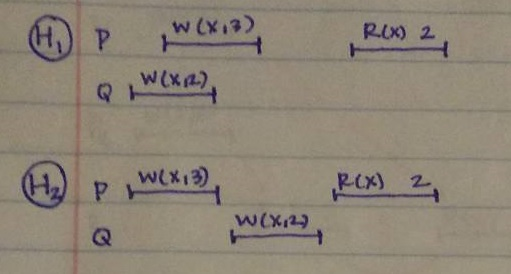
\includegraphics[width=90mm]{pic_1.jpg}
\caption{Two equivalent histories \label{overflow}}
\end{figure}
The processes in both concurrent histories are equivalent, but not identical since (H,\textless\textsubscript{H}) is not the same. In this example the three operations are permuted.

\section{Lamport’s Sequential Consistency}

A concurrent history (H,\textless\textsubscript{H}) is sequentially consistent if there exists a legal sequential history S such that:
1.	S is equivalent to H         2.	S preserves the process order in (H,\textless\textsubscript{H})

\begin{figure}[ht!]
\centering
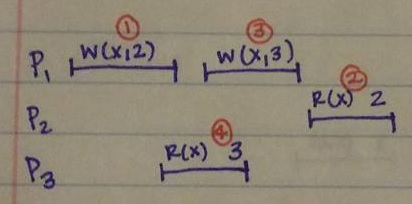
\includegraphics[width=90mm]{pic_3.jpg}
\caption{A sample sequential consistency \label{overflow}}
\end{figure}
Order across processes do not matter. Both histories from figure 11.1 are sequentially consistent.
\begin{figure}[ht!]
\centering
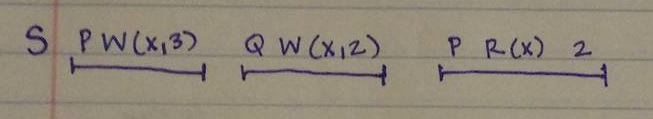
\includegraphics[width=90mm]{pic_2.jpg}
\caption{Sequential consistency of figure 11.1 \label{overflow}}
\end{figure}
\begin{figure}[ht!]
\centering
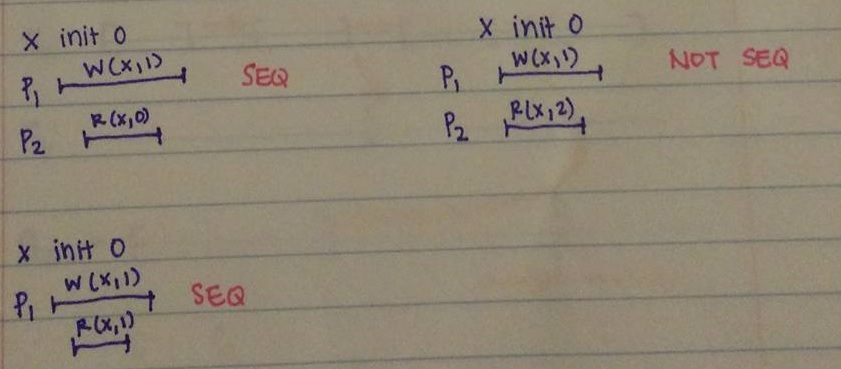
\includegraphics[width=90mm]{pic_7.jpg}
\caption{Sequential consistency example 1 \label{overflow}}
\end{figure}
\begin{figure}[ht!]
\centering
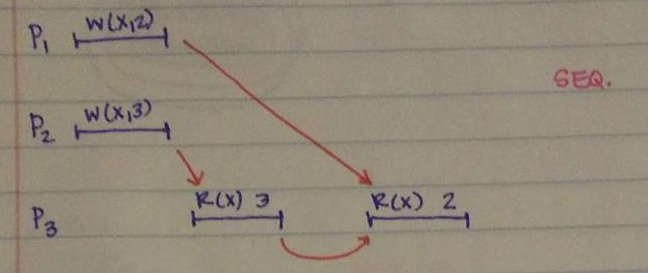
\includegraphics[width=90mm]{pic_5.jpg}
\caption{Sequential consistency example 2 \label{overflow}}
\end{figure}


\subsection{Not Sequential Consistency}

To show that it is not sequentially consistent, you show there is not any way to be sequentially consistent by either:

1.	The brute force method where you try out every combination for a case analysis
\begin{figure}[ht!]
\centering
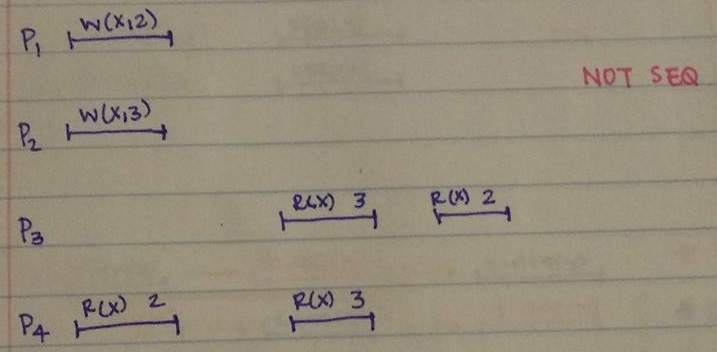
\includegraphics[width=90mm]{pic_6.jpg}
\caption{Not sequentially consistent \label{overflow}}
\end{figure}

2.	Check if there is a cycle such that the order cannot be preserved.

\begin{figure}[ht!]
\centering
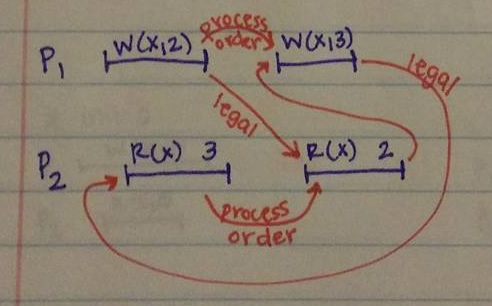
\includegraphics[width=90mm]{pic_4.jpg}
\caption{Not sequentially consistent cycle \label{overflow}}
\end{figure}


\subsection{Unfinished history}

Extend the unfinished by finishing up the history for a complete history that it is sequentially consistent

\section{Henlihy and Wing’s Consistency}

This correctness is stronger than sequential consistency and thus better for software purposes.
A history (H,\textless\textsubscript{H}) is linearizable/atomically consistent if there exists a  legal sequential history S such that:
1.	S is equivalent to H
2.	S preserves \textless\textsubscript{H}(the real time order)


\subsection{Linearizability and Sequential Consistency}

Theorem: H is LIN $\rightarrow$ H is SEQ

Proof: 
e \textless\textsubscript{process order} f $\rightarrow$  e \textless\textsubscript{H} f

The process-order is realtime order on the same process.

\subsection{Linearization Point}

That gives legality without operations. Linearization points should not match and must have some order.
\begin{figure}[ht!]
\centering
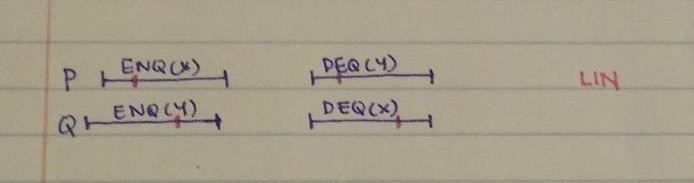
\includegraphics[width=90mm]{pic_10.jpg}
\caption{A linearizable history with linearization points\label{overflow}}
\end{figure}
\begin{figure}[ht!]
\centering
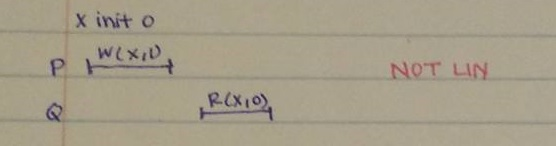
\includegraphics[width=90mm]{pic_9.jpg}
\caption{A non-linearizable history\label{overflow}}
\end{figure}
S1 = enq(x), eng(y) deq(x) deq(y)
S1 = enq(y), eng(x) deq(y) deq(x)

Theorem:
H is linearizable iff there exists linearization points for all operations such that the resulting sequence is legal and preserves the real time order.


\section{Linearizability and Sequential Consistency}

Suppose we have a legal program for queues and/or stacks and we join them.
\begin{figure}[ht!]
\centering
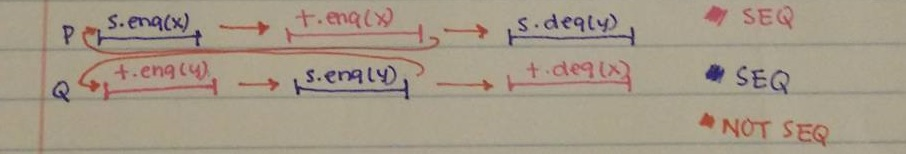
\includegraphics[width=90mm]{pic_11.jpg}
\caption{Illegal combination of two legal programs \label{overflow}}
\end{figure}

Defn: A consistency condition CONSISTENCY satisfies composability/locatlity if for all x: H $\vert$ x satisfies consistency $\longleftrightarrow$ H satisfies consistency

\subsection{Linearizability and Composability}

Theorem: LIN satisfies COMPOSABILITY

Proof: 

Claim: The graph stays acyclic. Two types of arrows
\begin{figure}[ht!]
\centering
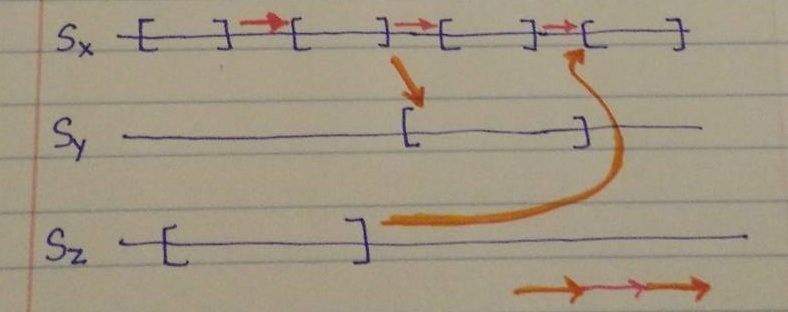
\includegraphics[width=90mm]{pic_12.jpg}
\caption{Linearizability cycle \label{overflow}}
\end{figure}
e \textless\textsubscript{H} f resp(e) occurred before inv(f)
f \textless\textsubscript{n} g resp(f) occurred before inv(g)
g \textless\textsubscript{H} h resp(g) occurred before inv(h)
By transitivity $\rightarrow$ resp(e) occurred before inv(h)
if any cycle $\rightarrow$ then to begin with thus no cycle
Thus, with a cycle we are not sequentially consistent.

\section{Other types of consistency}

Causal consistency,
FIFO consistency,
Entry Consistency
\begin{figure}[ht!]
\centering
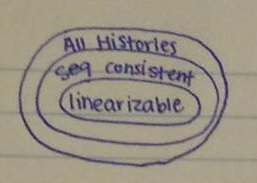
\includegraphics[width=90mm]{pic_8.jpg}
\caption{Consistency circles \label{overflow}}
\end{figure}

\subsection{Consistency Tradeoffs}

Stronger consistency gaurantees ease of programs, however this causes a loss of performance.


\section*{References}
\beginrefs
\bibentry{1}{\sc Vijay K Garg}, Multicore Computing, The University of Texas at Austin. September
2016.

\endrefs


\end{document}





